\subsubsection{About}

SVM (Support Vector Machines) works by, simply put, dividing the data into categories \parencite{wang2005comparison}. This is done with "drawing the line" on the grid.

Example bellow showcases how two classes are divided by the model.
\begin{figure}[H]
    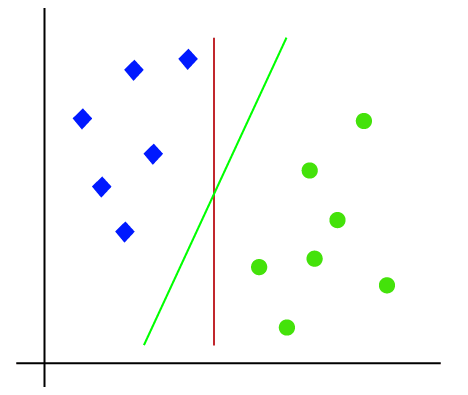
\includegraphics[scale=0.50]{img/Classification/SVM.png}
    \centering
    \caption{SVM example \parencite{web:Rocketloop}}
    \label{fig:SVM}
\end{figure}

As with decision tree, we have used same library in order to get SVM model.